\subsection{Cluster Labelling}
\label{sec:impl_cluster_labeling}

We implemented our own cluster labelling methods, which consider the most important features of a cluster.
They will be explained using the following example:
The current feature is ``length of blog posts'' and we have three clusters with the following values for the feature:
\begin{center}
\begin{tabular}{c|c|c}
  Cluster 1 & Cluster 2 & Cluster 3 \\ \hline
  0.7 & 1 & 0.1 \\
 \end{tabular}
\end{center}


\paragraph{Method 1}
For each feature and cluster, the highest and lowest value is determined.
Those clusters are then given the appropriate labels.

In the example cluster 2 has the highest value and gets the label ``longest blog posts''.
The label ``shortest blog posts'' is assigned to cluster 3, because this cluster has the lowest value.
Using this method only the most significant labels are set.
But a cluster may not obtain any label when it does not have any extreme features.


\paragraph{Method 2}
First, the average vector of all blog posts is calculated.
In a second step, the distance for each feature and cluster to that average vector is determined.
If the distance is over a certain threshold, the cluster is labelled.

The example is shown in Figure~\ref{fig:cluster_labeling_2}.
Because cluster 3 is not over the threshold, thus the length of the blog post is not significant for the cluster, no label is assigned to that cluster.
Cluster 1 and 2 are both over the threshold and obtain the label ``long blog posts''.
This method assigns more labels to clusters than method 1, but can also lead to clusters without any labels if all of a cluster's feature have average values.

\begin{figure}[ht]
	\centering
	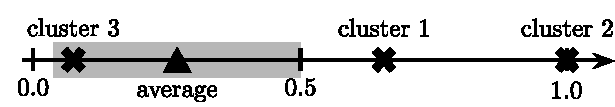
\includegraphics[width=0.6\textwidth]{images/cluster_labeling_2.pdf}
	\caption{Cluster labelling method 2: The distance of each cluster to the overall average blog posts is calculated. If the distance is below or over a certain threshold (shaded in grey), the cluster obtains a label. In this example a label is assigned to cluster 1 and 2.}
	\label{fig:cluster_labeling_2}
\end{figure}


\paragraph{Method 3}
As with method 2, we calculate the difference to the average for each cluster and feature.
However, we also normalize them to the total range this feature has for our data.
Then, we pick the $n$ most significant of these differences for each cluster and use them to label it.
Significance, in this case, is mostly determined by how great the deviation from the average is: The larger the deviation the higher the significance.
The only exception to this is that being close to to the average is considered slightly more significant than being fairly close to it.

In our example, clusters 2 and 3 would most likely obtain the label ``longest'' or ``shortest blog posts'' respectively.
Cluster 1 on the other hand would be eligible for the low significance label ``average length blog posts'' but might not receive it if it has $n$ more significant labels.
With this method, every cluster is guaranteed to obtain a set number of labels, even if it has no features that deviate from the average. \\


Our final implementation uses method 3 since it guarantees us a set number of feature labels for each cluster.
We found that providing five labels for each cluster was usually enough to describe them in a unique way while still being few enough not to confuse the user.
Thus, our final implementation of method 3 lets each cluster obtain five different labels, so $n$ was set to 5.
